\chapter{Methodology}
This chapter describes the data collection of merge samples and the empirical evaluation of the intentions language and intention-based variant integration tool \tooln.

\section{Data collection}
Two methods for collecting data from open-source ecosystems have been used, one for gathering a ground truth for how variant integration is achieved through merging, and one for procuring smaller scale authentic integration candidates scenarios. We denote the output of the former method \textit{merge examples} and the output of the latter method \textit{integration scenarios}. The merge examples are used for understanding the context and execution of the variant-integrating merge. They can also be replayed for validation, since they represent the ground truth outcome of the two merge parents. As such, the merge examples serve as an important validation tool. However, since the merge examples are extracted from a three-way merging tool, they are disadvantageous for replaying in \tooln, since three-way information is not available in that environment. To this end, we use the integration scenarios, which are free from three-way contamination, but are instead taken out of their context and are scaled down.

\subsection{Collecting ground truth merge examples}
To identify and validate the integration intentions we analyze variant-related merges and extract common patterns. We begin by retrieving all merges and discard those that merged without conflicts. Merge instances with conflicts signify a syntactic conflict which is an indicator of potential feature integration. In order to investigate further, for each of these merges, we save the state of the entire source tree at the following revisions:  
a) after the merge, i.e. the \textit{result},
b) in the first parent, i.e. the \textit{head}, and
c) in the second parent, the \textit{merge head}. We call this triple of source trees the \textit{related artifacts} of the merge, the relationship between its parts is shown in Figure \ref{intentions:mergespace}. Retaining and inspecting the source trees of the parents allows for insights to be gathered, and in particular the ability to replay the merge in order to reach the known result. Note that the search space, the entire set of merges encompasses \textit{all} merges, that is, merges that occurred in a fork but were subsequently merged into the mainline are also included. We do \textit{not} use the \texttt{-{}-first-parent} option to Git, which would discard such further merges residing in recursive parents, and instead use only the first parent when finding merges. The merges that are included by this broader search scope originate either from ordinary feature merging or from pull requests where the branch of the requester is out of date.%\todo{Figure showing ABL feature integration and Deltabot feature integration.}

When the related artifacts from each merge have been collected, we inspect them and discard merges with any of the following properties: 
a) all conflicts occurred in non-source-code artifacts, b) at least one artifact cannot be compiled, c) there are only whitespace changes between the merge parents, or d) contain some project-specific uninteresting changes (see Section \ref{data-coll-res} for examples of what \textit{uninteresting} entails in practice).

\begin{figure}[ht]
    \centering
    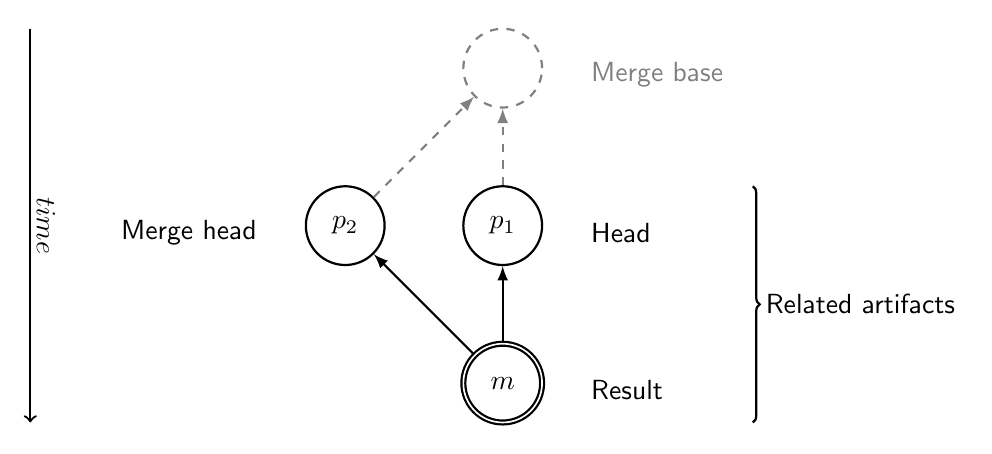
\begin{tikzpicture}
        \tikzset{every node/.append style={font=\sffamily}}
        \tikzstyle{linez} = [thick]
        \tikzstyle{commit} = [shape=circle,draw=black, minimum size=1cm, linez]
        \tikzstyle{ancestor} = [draw=gray, dashed]
        \tikzstyle{messager} = [xshift=1cm, yshift=-0.6cm, anchor=west]
        \tikzstyle{messagel} = [xshift=-1cm, yshift=-0.6cm, anchor=east]

        \node[commit, double, label={[messager]Result}] (res) at (0,0) {$m$};
        \node[commit, label={[messager]Head}] (ba) at (0,2) {$p_1$};
        \node[commit, label={[messagel]Merge head}] (re) at (-2,2) {$p_2$};
        \node[commit, ancestor, label={[messager, color=gray]Merge base}] (an) at (0,4) {};
        
        \draw[thick, decoration={brace,mirror,raise=5pt},decorate] (3,-0.5) -- node[right=6pt] {Related artifacts} (3, 2.5);
        
        \draw[thick,->] (-6,4.5) to node[pos=0.5, xshift=0.2cm, rotate=-90] {$time$} (-6,-0.5);
        
        \draw [->, -latex, linez] (res) -- (ba);
        \draw [->, -latex, linez] (res) -- (re);
        \draw [->, -latex, ancestor, linez] (re) -- (an);
        \draw [->, -latex, ancestor, linez] (ba) -- (an);
        % NOTE: There is a bug in tikz with -latex arrows and colors. The arrows should therefore be drawn last, otherwise the colors of the arrowheads can mess up.
        
    \end{tikzpicture}
    \caption{Merge commit context. The merge commit $m$ has two parents, $p_1$ and $p_2$. The entire state of the source tree is gathered, in these three commits. These source sets are denoted \textit{result}, \textit{head}, and \textit{merge head}. This triple of source tree sets constitute the \textit{related artifacts} of the commit $m$.}
    \label{intentions:mergespace}
\end{figure}

\subsection{Creating authentic integration scenarios}
Since the merge examples discussed in the previous section would be replayed without three-way information, and are potentially very large, it is desirable to have a neutral and concentrated basis for task creation, referred to as \textit{integration scenarios}. The contents of integration scenarios are based on variant integration examples from the ecosystem (mainline and forks), with the diff chunks consolidated so that there is not an abundance of code with no changes. Additionally, changes may originate from several different source files, and can have syntax and semantics changed. The structure of the source chunks, and the conflict resolution ground truth is left intact.

\section{Internal evaluation}
For the proof-of-concept internal evaluation using the three tool developers, we use code from Marlin. There are two types of tasks: to replay merge examples, and to merge forks with the mainline. The characteristics of these tasks are shown in Table \ref{tab:internalchar}, where Blocks denotes the number of changed chunks according to \texttt{diff}. The merge tasks are chosen from the set of merge tasks in Marlin, and the forks are chosen based on the findings of St\u{a}nciulescu et al. \cite{stanciulescu2015}. It does not matter whether they are still actively maintained or not, because we set the task at the \head of the fork, and then compare with the latest common ancestor commit \texttt{\#ancestor} between fork and mainline, and devise a resolution strategy for the task.

Each developer performs 3-4 tasks, at least one of each kind. The integration task is performed in the manual unstructured Eclipse CDT and \tooln. The number of edit operations required per task in each editor is saved for analysis, as is the resulting output file. Each task consists of a number of input files from the two variants being integrated, together with a textual description of what the integration goal is. The output files are checked for syntax errors and bugs introduced.

\begin{table}[ht]
    \centering
    \caption{Internal evaluation task characteristics.}
    \label{tab:internalchar}
    \begin{tabular}{lll|lll}
\hline\hline
\textbf{Name} & \textbf{Type} & \textbf{Files} & \textbf{$\pm$ Blocks} & \textbf{$\pm$ \texttt{\#ifdef}s} & \textbf{$\pm$ Lines} \\
%Name & Type & Files& $\pm$ Blocks & $\pm$ \texttt{\#ifdef}s & $\pm$ Lines\\
\hline
08856d9      & Merge     & 1 & 17    & 4     & 263   \\
17de96a      & Merge     & 1 & 34    & 18    & 256   \\
2daa859      & Merge     & 2 & 141 & 79      & 889   \\
3116271      & Merge     & 1 & 6     & 0     & 51    \\
373f3ec      & Merge     & 1 & 108 & 60      & 718   \\
46f80e8      & Merge     & 1 & 2     & 0     & 4     \\
47c1ea7      & Merge     & 1 & 188   & 195   & 2,343 \\
\hline
esenapaj     & Fork         & 3 & 98    & 118   & 734   \\
jcrocholl    & Fork         & 1 & 39    & 27    & 290   \\
STM32        & Fork         & 3 & 153   & 26    & 423   \\
\hline\hline
    \end{tabular}
\end{table}

\section{Controlled experiment}
This sections describes the experimental design and setup, together with the integration scenarios from \busybox~and \vim, that are the subject programs in the experiment.
%Designed based on Melo et al \cite{melo2016latin} (also the subsequent paper from 2017). % -- it has really good related work that can be used to show that the preprocessor (and configurations) are often erroneous.

\subsection{Objective}
To establish the beneficence of an intention-based integration strategy in general, and INCLINE in particular, we evaluate the tool using subject programs from other sources than Marlin, since Marlin was used to elicit the set of intentions. The purpose of the controlled experiment is to answer the following research questions:
\begin{enumerate}[label={Q\arabic*}]
    \setcounter{enumi}{1}
    \item \RQB
    \item \RQC
\end{enumerate}

\subsection{Treatments}
In order to study the beneficence of intention-based integration, we let each participant solve one task using the ordinary unstructured merge tool inside Eclipse CDT, and one task using \tooln. The two treatment levels are thus \textit{Eclipse CDT} \texttt{Ecl} and \textit{\tooln} \texttt{MPS}.

\subsection{Subjects}
Using the process for collecting authentic variant integration scenarios, we prepare two sample programs to be used in the experiment: \po, based on \busybox, and \pt, based on \vim. These two programs are created as condensed versions of the changeset of a particular fork variant, for brevity and comprehension during the experiment. This should be understood as selecting the most suited changes across the files, and placing them in a single file, in order to not waste valuable time for the participants on long blocks without any changes, as to keep the programs brief. Table \ref{method:charac} lists the characteristics of the subject programs. All measurements relate to the integrated model of the programs, with \textit{Integrated LOC} signifying the LOC. \textit{Chunks and excluded chunks} shows the number of selected variation points from the full changeset to be in the program, and the excluded count. \textit{Variable LOC} (VLOC) is LOC count of lines under a presence condition containing the literal \texttt{FORK} -- i.e. the LOC count in variant branches in the integrated model -- in particular, these are the lines that must be manipulated by the participants.

We choose \busybox~ and \vim~ as representative subjects because they are highly-configurable open source systems, and have been subjects in previous studies \cite{berger2013study}, \cite{liebig2010preprocessor}, \cite{liebig2011discipline}.

\begin{table}[ht]
    \centering
    \caption{Characteristics of the programs \po~and \pt.}
    \label{method:charac}
    \begin{tabular}{c l l l l l}
    \hline
    \hline
        \textbf{Prg} & \textbf{Origin} & \textbf{Integ. LOC} & \textbf{\#chunks} & \textbf{\#excl. chunks} & \textbf{VLOC}\\\hline
        \po & \busybox  & 73 & 8 & - & 36\\\hline
        \pt & \vim      & 49 & 5 & - & 29\\
        \hline
        \hline
    \end{tabular}
\end{table}

\subsection{Design}
The experiment is a 2$\times$2 within-subjects counterbalanced Latin square design \cite{box}. Each developer performs two tasks with the treatment order and program order randomized in order to reduce learning effects. Table \ref{method:ls1} shows the base Latin square.
Since developers are assigned at random, no further permutation of the treatments in the 2$\times$2 Latin square is required, since the two other possible combinations would be redundant with respect to program order and treatment. The benefit of a within-subject design is the reduced number of required subjects participating in the experiment, but at the cost of carryover effects, in this case particularly learning effects. We therefore employ a counterbalanced design, where the order of the tasks is randomized.

\begin{table}[ht]
\centering
\caption{Latin Square (2$\times$2).}
\label{method:ls1}
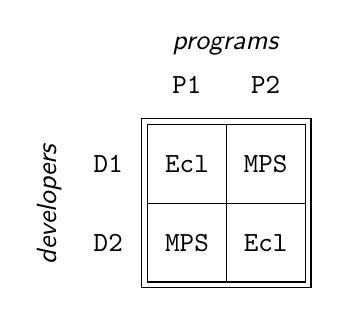
\begin{tikzpicture}
    \node[minimum size=1cm,draw=black] (sba) at (0,0) {\texttt{MPS}};
    \node[minimum size=1cm,draw=black] (sbb) at (1,0) {\texttt{Ecl}};
    \node[minimum size=1cm,draw=black] (saa) at (0,1) {\texttt{Ecl}};
    \node[minimum size=1cm,draw=black] (sab) at (1,1) {\texttt{MPS}};
    \node[minimum size=1cm] (ld1) at (-1,1) {\texttt{D1}};
    \node[minimum size=1cm] (ld2) at (-1,0) {\texttt{D2}};
    \node[minimum size=1cm] (lp1) at (0,2) {\texttt{P1}};
    \node[minimum size=1cm] (lp2) at (1,2) {\texttt{P2}};
    
    \node[minimum size=2.15cm,draw=black] (square) at (0.5,0.5) {};
    \node[] (lprog) at (0.5, 2.5) {\textit{programs}};
    \node[rotate=90] (ldevs) at (-1.75, 0.5) {\textit{developers}};
\end{tikzpicture}
\end{table}

\anova~is used to test the significance of differences between the treatments. The prerequisites for an \anova~test are normality, homoscedasticity, and unit-treatment additivity. These assumptions are tested using the Box Cox, Bartlett and Tukey additivity test.

\subsection{Execution}
%Before running the actual experiment, we executed a pilot study with the authors of \cite{lillack2017intentions}, in order to assess the presentation of the tasks and the distribution of our tooling.
Before the experiment, we elicit the background of the participants through a questionnaire containing Likert-scale questions about how familiar they are with certain programming languages and merging techniques and tools.

Introductions to each task are done by screen cast, to ensure that all participants receive the same introduction, regardless of which session they attend.

After the tasks are completed, participants fill in an exit questionnaire with closed and open-ended questions about their perceptions of \tooln~and intention-based integration compared to regular, unstructured integration in a merge tool. 

Semi-structured debriefing interviews ask about benefits and challenges of intention-based integration, and improvements to it.
